\chapter{Aktualny stan projektu Gerbil}

\index{MVC} \section{Wzorzec MVC}

Aplikacja Gerbil jest zaprojektowana według wzorca MVC (Model-View-Controller) z~wykorzystaniem platformy Qt. MVC jest wzorcem architektonicznym używanym często do tworzenia interfejsów użytkownika. Podstawą MVC są trzy obiekty:
\begin{itemize}
	\item model -- komponent odpowiedzialny za serwowanie danych;
	\item widok -- komponent odpowiedzialny za wizualizację danych;
	\item kontroler -- komponent definiujący logikę, za pomocą której interfejs użytkownika odpowiada na jego żądania.
\end{itemize}
Podział tych ról można zaobserwować na rysunku ~\ref{fig:mvc}.

\begin{figure}[ht]
	\centering
	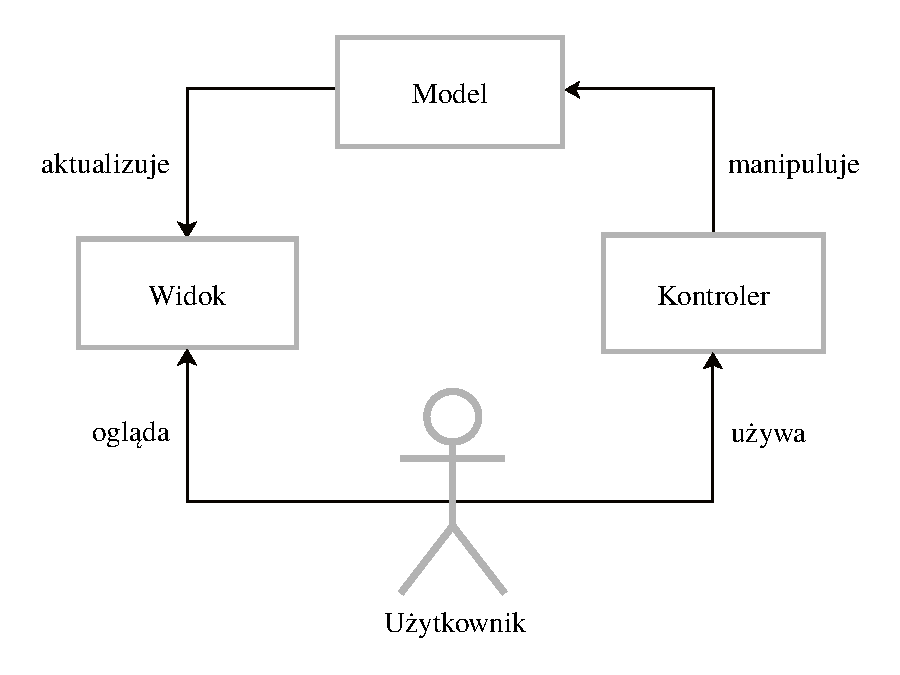
\includegraphics[width=0.7\linewidth]{rys04/mvc}
	\caption{Podział ról we wzorcu architektonicznym MVC}
	\label{fig:mvc}	
\end{figure}

Dzięki wykorzystaniu tego wzorca sposób przechowywania danych nie ma wpływu na to jak są one przedstawione użytkownikowi~\cite{Qtdoc}.

\section {Architektura aplikacji Gerbil}

W aplikacji Gerbil wzorzec MVC zastosowano w~sposób klasyczny: 
\begin{itemize}
	\item modele są odpowiedzialne za obliczenia danych oraz sygnalizowanie pojawienia się ich nowej wersji;
	\item widoki wyświetlają dane;
	\item kontrolery zajmują się kojarzeniem akcji użytkownika z~konkretną funkcjonalnością modelu.
\end{itemize}

Dodatkowo w~aplikacji występuje wątek roboczy. W nim uruchomiona jest kolejka zadań. Zadanie (obiekt klasy \lstinline$Task$) jest komponentem realizującym wykonanie czasochłonnego algorytmu analizy danych. Modele tworzą zadania i~przekazują je do kolejki. Kolejka przyjmuje zadania i~wykonuje je po kolei. W ten sposób skomplikowane obliczenia nie blokują wątku GUI, który pozostaje przez cały czas responsywny.

W takiej architekturze pojawia się problem dostępu do danych, ponieważ dwa wątki (wątek GUI, w~którym znajdują się komponenty MVC, oraz wątek roboczy, w~którym wykonywane są zadania) próbują uzyskać dostęp do tych samych danych. Zadania wykonywane w~tle powinny w~bezpieczny sposób dokonywać zapisu danych. Widoki zaś powinny być w~stanie bezawaryjnie wizualizować dane oraz dbać o~aktualność prezentowanych danych.

\subsection{Wady architektury}

System ten jest mocno zdecentralizowany. Na barkach kontrolerów spoczywa odpowiedzialność odpowiedniej propagacji sygnałów informujących o~nowej wersji danych, inwalidacji danych, jak również zapytań o~dokonanie nowych obliczeń. Prowadzi to do:
\begin{itemize}
	\item zaciemnienia kodu źródłowego zbędnymi instrukcjami warunkowymi,
	\item zignorowania pewnych sygnałów,
	\item podjęcia niewłaściwej decyzji.
\end{itemize}

Zarządzanie zadaniami również jest wadliwe. W przypadku gdy użytkownik poprzez interakcję z~systemem zleci wykonanie na raz kilku zadań dokonujących obliczeń na tych samych danych, system może zachować się w~sposób nieoczekiwany. Prowadzi to do zakończenia aplikacji z~powodu naruszenia ochrony pamięci. Nowa wersja systemu powinna w~najgorszym wypadku zakolejkować te zadania i~wykonać jedno po drugim.

Wiele komponentów interfejsu użytkownika przechowuje własne uchwyty do danych oraz ewentualnie muteks. Wobec tego same dokonują synchronizacji lub nie robią tego wcale. Nieprzemyślany model doprowadził do wielu patologii. Przykład stanowi używanie współdzielonych wskaźników do przekazywania danych, podczas gdy dane te z~założenia powinny być współdzielone.

\subsubsection{Konkluzja}

Aktualny model współdzielonych danych, w~powiązaniu z~modelem zarządzania nimi nie gwarantuje bezpiecznego dostępu do danych ani prawidłowego przebiegu procesu wykonania zadań. Biorąc pod uwagę wyżej wymienione problemy nowy mechanizm zarządzania danymi oraz procesem wykonania powinien: 
\begin{itemize}
	\item posiadać wewnętrzny mechanizm synchronizacji dostępu do danych,
	\item gwarantować bezpieczny dostęp do współdzielonych danych,
	\item gwarantować bezpieczne wykonanie zadań w~tle,
	\item gwarantować prawidłową kolejność procesu przetwarzania danych,
	\item posiadać scentralizowany mechanizm propagacji sygnałów,
	\item prawidłowo propagować informację o~dostępności nowej wersji danych,
	\item prawidłowo propagować informację o~żądaniu obliczeń nowych danych.
\end{itemize}





